\newpage
\section{Manual de Usuario}
\label{sec:manual_usuario}

El presente manual tiene como objetivo proporcionar una guía visual, estructurada y detallada para el usuario final de MoodNest. A través de este documento se explican en profundidad los flujos de interacción de la plataforma, detallando las acciones disponibles en cada pantalla y el comportamiento de los elementos visuales que componen la interfaz.

\subsection{Acceso Público y Gestión de Autenticación}

El ciclo de vida del usuario en MoodNest comienza en la periferia pública de la plataforma, diseñada bajo principios de mínima fricción cognitiva para incentivar el registro.

\subsubsection{Pantalla de Bienvenida y Onboarding}

Al acceder a la URL principal, el sistema renderiza la interfaz pública de bienvenida. Esta pantalla expone la propuesta de valor de MoodNest mediante un diseño minimalista y limpio (ver Figura~\ref{fig:bienvenida}).

\begin{figure}[H]
    \centering
    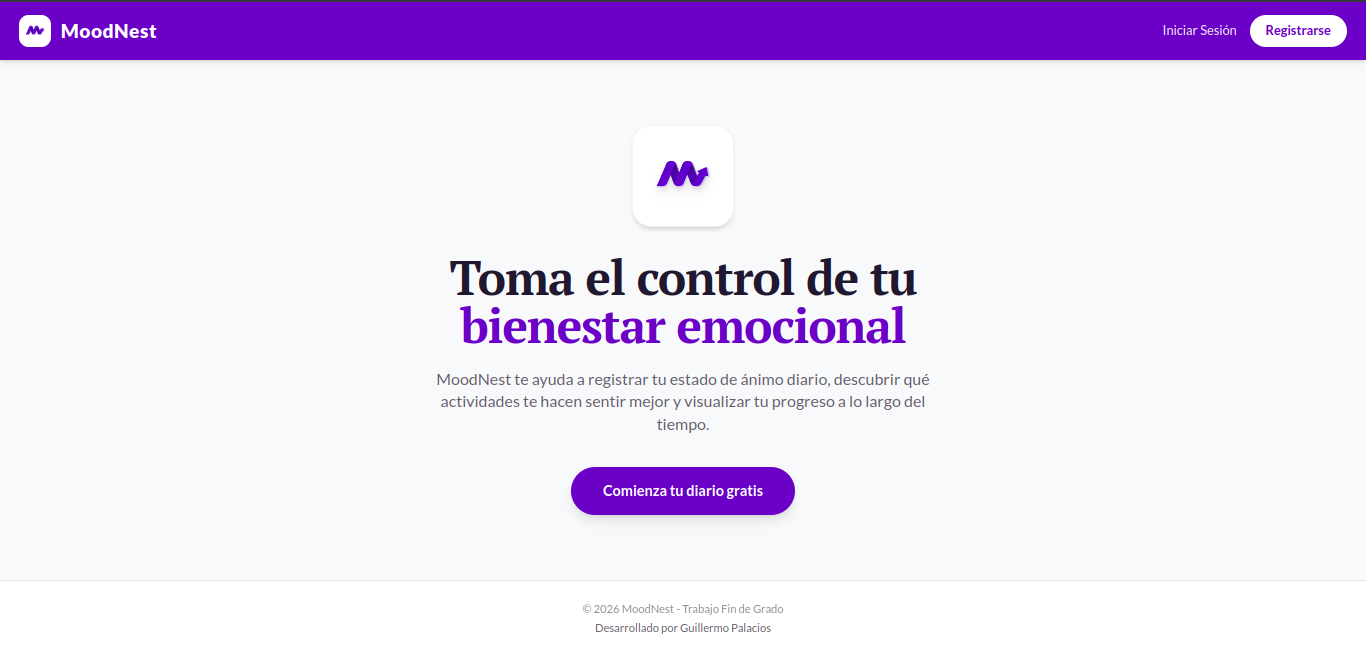
\includegraphics[width=0.85\textwidth]{Imagenes/pantalla_bienvenida.png}
    \caption{Pantalla de Bienvenida pública de MoodNest.}
    \label{fig:bienvenida}
\end{figure}

Los componentes interactivos clave distribuidos en esta vista son:
\begin{itemize}
    \item \textbf{Barra de Navegación:} Ubicada en la zona superior, expone de manera persistente dos botones de acción de alta visibilidad: ``Iniciar Sesión'' y ``Registrarse''.
    \item \textbf{Llamada a la Acción Principal:} En el centro de la pantalla se dispone el botón destacado ``Comienza tu diario gratis''. Al pulsar en este botón, el usuario será redirigido al apartado de registro para dar inicio a su aventura en MoodNest.
\end{itemize}

\subsubsection{Formularios de Acceso y Registro de Cuentas}

Al interactuar con los botones de ``Iniciar Sesión'' o ``Registrarse'', el usuario será redirigido a los apartados correspondientes para, por un lado, acceder a MoodNest con una cuenta ya existente en el sistema (Iniciar Sesión (ver Figura~\ref{fig:login})), o por otro lado, crear una nueva cuenta en el sistema (Registrarse (ver Figura~\ref{fig:registro})).

\begin{figure}[H]
    \centering
    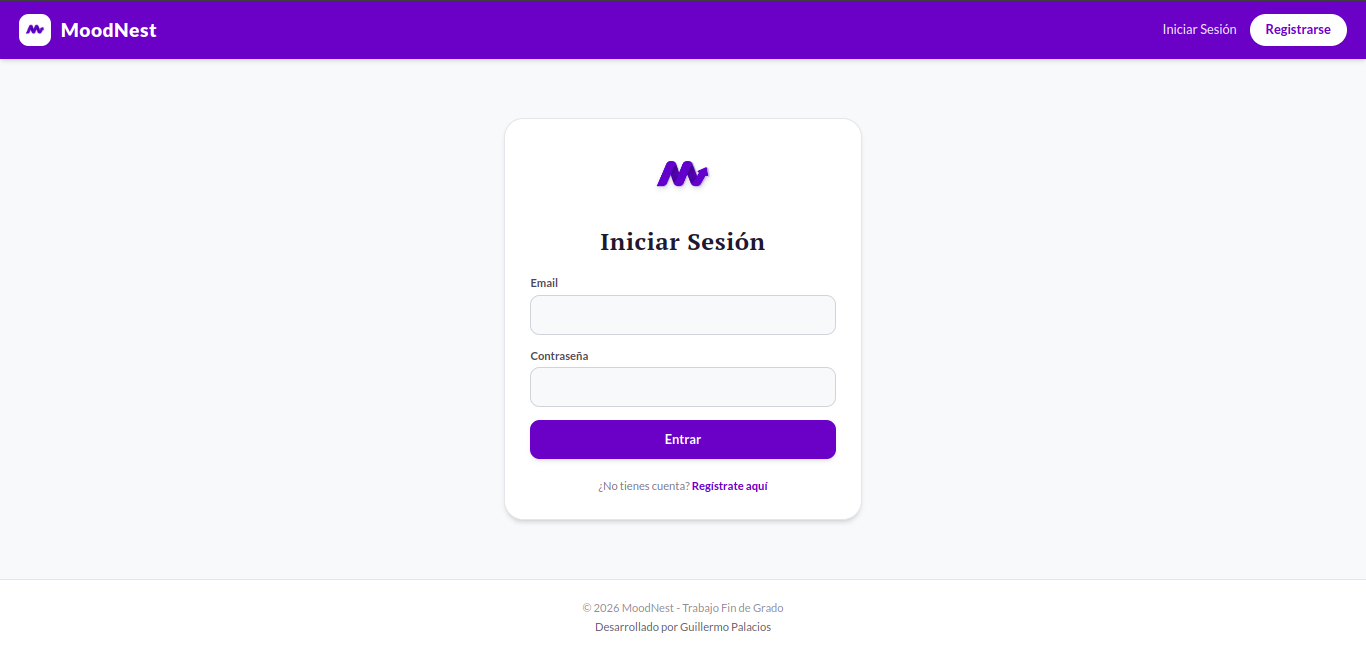
\includegraphics[width=0.85\textwidth]{Imagenes/pantalla_iniciar_sesion.png}
    \caption{Interfaz de Inicio de Sesión de MoodNest.}
    \label{fig:login}
\end{figure}

\begin{figure}[H]
    \centering
    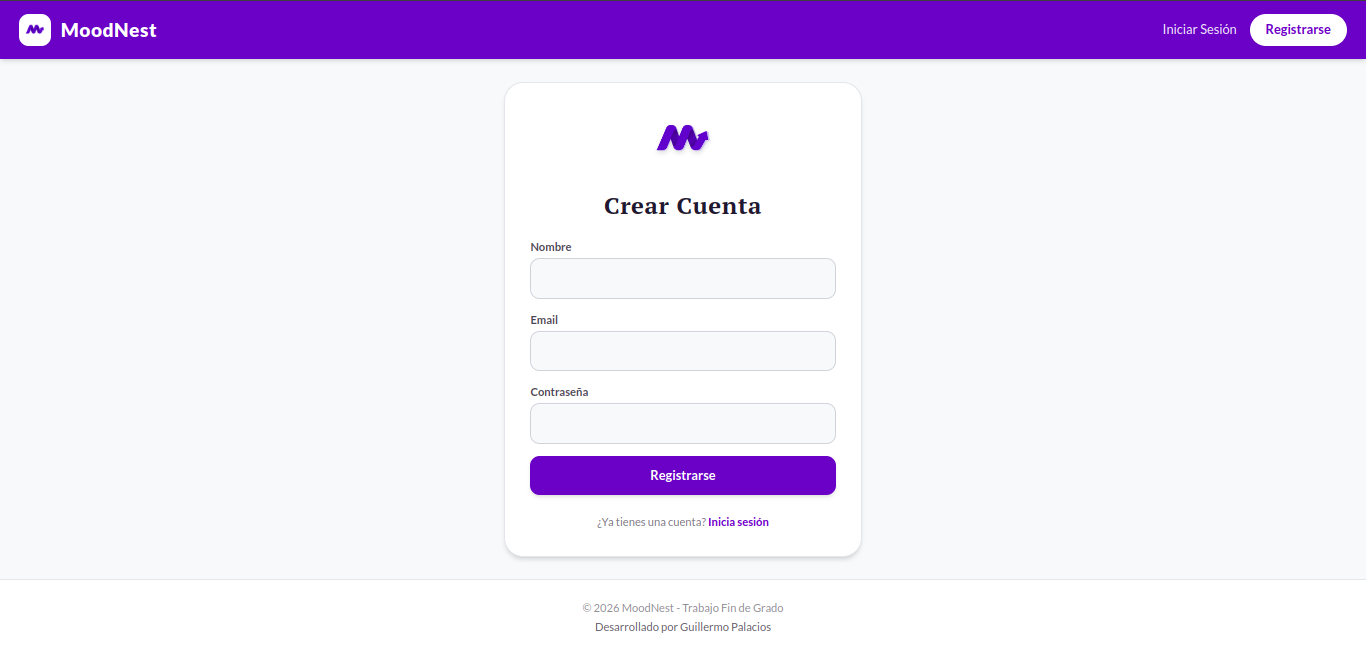
\includegraphics[width=0.85\textwidth]{Imagenes/pantalla_crear_cuenta.png}
    \caption{Interfaz de Registro de Usuario en MoodNest.}
    \label{fig:registro}
\end{figure}

Ambas vistas se estructuran mediante módulos de captura de datos validados en tiempo real:
\begin{itemize}
    \item \textbf{Campos de Entrada:} En la pantalla de inicio de sesión se solicitan obligatoriamente los campos de correo electrónico y contraseña, mientras que en la pantalla de registro se incluye también el campo de ``Nombre'', el cual representa el apodo que el usuario quiere tener dentro de MoodNest.
    \item \textbf{Enlaces de Interconexión Cruzada:} Con el fin de facilitar la navegación al usuario, la base de cada tarjeta incluye un enlace de redirección, facilitando al usuario la creación de una nueva cuenta o el acceso con una ya existente (``¿No tienes cuenta? Regístrate aquí'' y ``¿Ya tienes cuenta? Inicia sesión''), vinculando ambos estados de forma directa sin requerir volver a la página de bienvenida.
\end{itemize}

\subsection{El Panel Principal (Dashboard) Inicial}

Una vez que el usuario accede de forma exitosa en MoodNest, ya sea iniciando sesión o registrándose, será dirigido a su panel principal donde podrá comenzar su aventura en MoodNest (ver Figura~\ref{fig:dashboard_inicial}).

\begin{figure}[H]
    \centering
    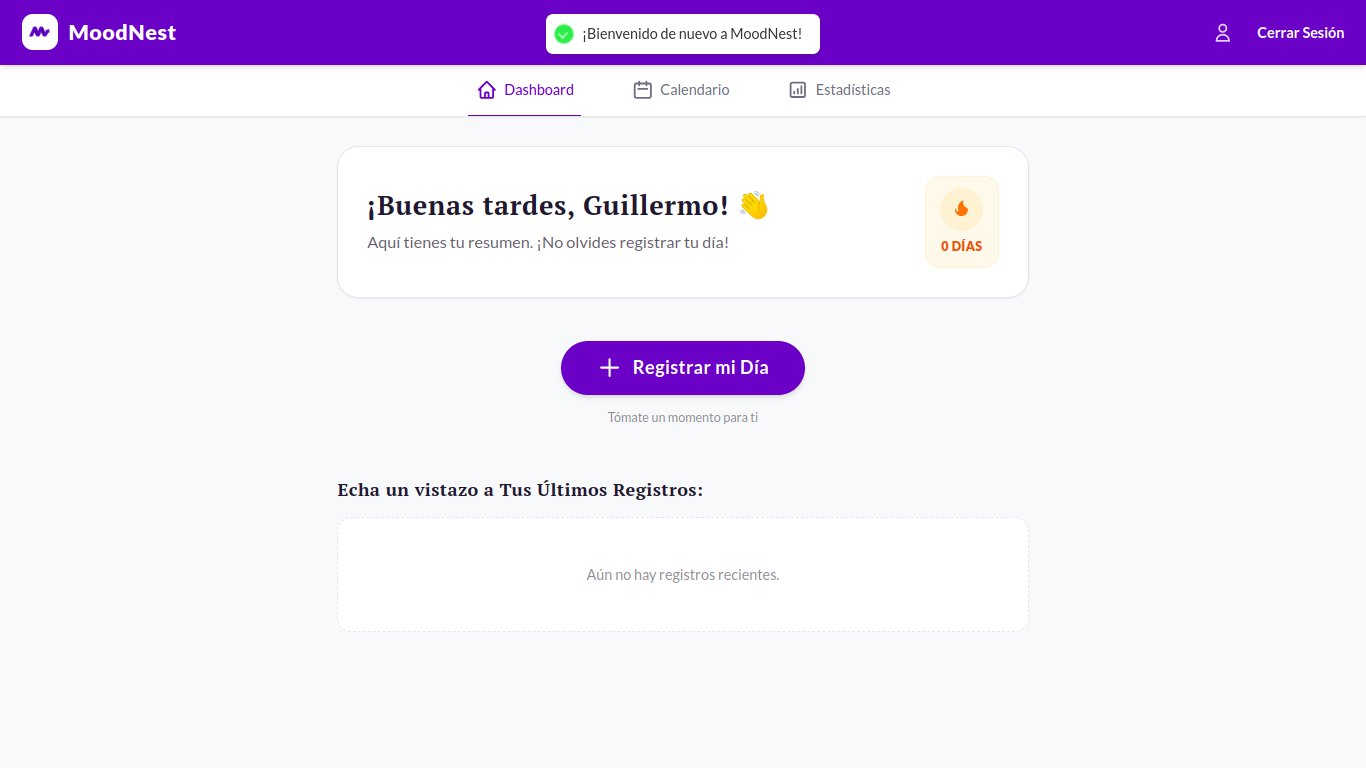
\includegraphics[width=0.85\textwidth]{Imagenes/pantalla_dashboard_inicial.png}
    \caption{Vista general del Dashboard Inicial tras el primer acceso.}
    \label{fig:dashboard_inicial}
\end{figure}

En este escenario de primera toma de contacto, destacan los siguientes elementos reactivos:
\begin{itemize}
    \item \textbf{Notificación Reactiva de Bienvenida:} Cuando el usuario interactúa con MoodNest, recibirá retroalimentación mediante notificaciones flotantes, visibles en la parte superior central de la pantalla.
    \item \textbf{Menú de Navegación Interna:} Dispuesto de forma horizontal justo debajo de la barra de navegación superior. Es el encargado de permitir al usuario moverse con facilidad entre las distintas pantallas de MoodNest (Dashboard (Actual), Calendario y Estadísticas).
    \item \textbf{Saludo Dinámico y Racha:} En la propia pantalla del Dashboard, destaca su saludo dinámico, el cual varía según la franja horaria del usuario y su nombre dentro de MoodNest y como subtítulo se muestra un mensaje que advierte al usuario de que el día está pendiente de registro. Justo en la parte derecha observaremos la racha actualizada del usuario, la cual representa el número de días registrados consecutivamente hasta la fecha actual.
    \item \textbf{Control Central de Inserción:} Se presenta el botón de gran formato ``Registrar mi Día'' como el elemento con mayor peso visual y el que permite crear los registros diarios al usuario.
\end{itemize}

\subsection{Formulario de Registro Diario y Gestión de Etiquetas}

Al presionar el botón central, la interfaz despliega una ventana modal con el formulario completo para rellenar el estado de ánimo diario del usuario. En la Figura~\ref{fig:reg_inicial} se observa el formulario inicial en blanco, mientras que en la Figura~\ref{fig:reg_rellenado} se muestra ya rellenado, con sus etiquetas asociadas y su comentario, siendo estos dos últimos opcionales.

\begin{figure}[H]
    \centering
    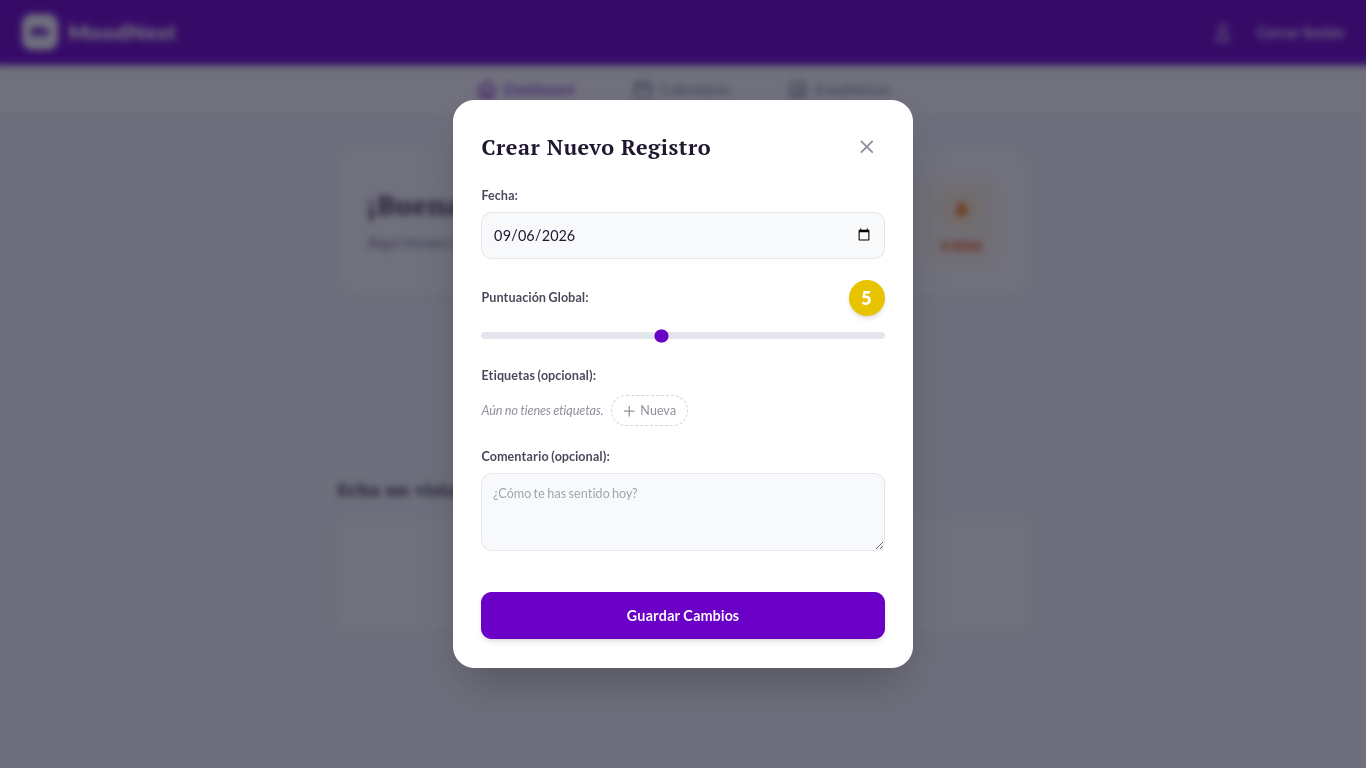
\includegraphics[width=0.85\textwidth]{Imagenes/pantalla_crear_registro_inicial.png}
    \caption{Formulario de registro diario en estado inicial.}
    \label{fig:reg_inicial}
\end{figure}

\begin{figure}[H]
    \centering
    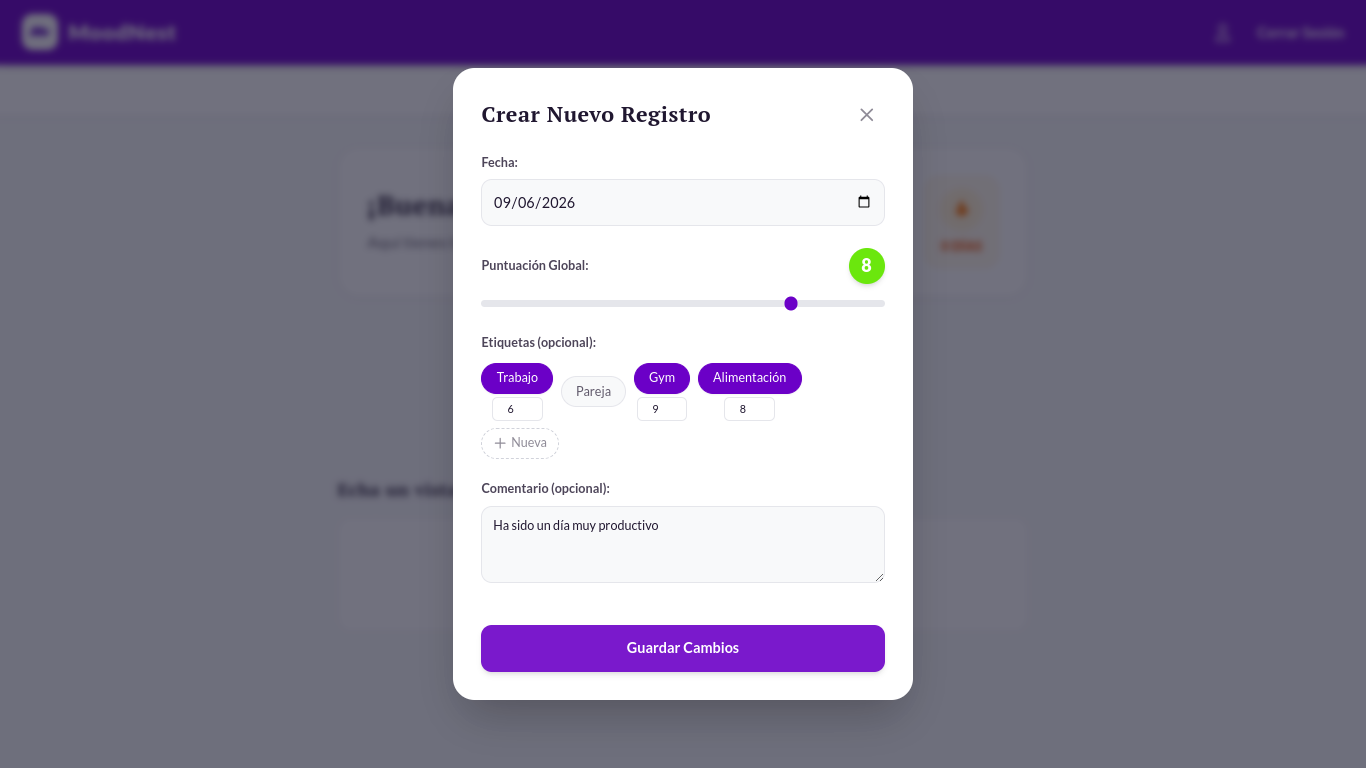
\includegraphics[width=0.85\textwidth]{Imagenes/pantalla_crear_registro_rellenado.png}
    \caption{Formulario de registro diario rellenado con sub-notas y tags evaluados.}
    \label{fig:reg_rellenado}
\end{figure}

El formulario se compone de cuatro áreas funcionales:
\begin{enumerate}
    \item \textbf{Selector Temporal de Fecha:} Preselecciona automáticamente el día actual. Permite su modificación para rellenar jornadas del pasado, bloqueando sin embargo la selección de fechas futuras.
    \item \textbf{Deslizador de Puntuación Global:} Control deslizante del 1 al 10. Al ser manipulado, el indicador numérico cambia reactivamente de color siguiendo la escala semántica emocional.
    \item \textbf{Cuadro de Selección de Etiquetas:} Las etiquetas han sido pensadas para que el usuario pueda asociar actividades, emociones, situaciones, personas, etc. Cualquier cosa que ayude a representar mejor su día. Si el usuario aún no tiene etiquetas creadas puede crearlas en el momento rápidamente y si ya tiene etiquetas creadas puede asociarlas o desactivarlas (Si ya están asociadas) de su día simplemente haciendo clic sobre ellas. Además al asociar una etiqueta, será posible la opción de incluirle una puntuación a dicha etiqueta de forma completamente opcional.
    \item \textbf{Comentario Textual:} Área libre completamente opcional para aquellas anotaciones extra o de diario que el usuario quiera incluir sobre su día.
\end{enumerate}

\subsection{Panel Principal (Dashboard) Post-Registro}

Una vez que el usuario presiona ``Guardar Registro'', la información es procesada y guardada en el historial del usuario. De inmediato, la aplicación actualiza el panel principal para reflejar el cambio de estado (ver Figura~\ref{fig:dashboard_post}).

\begin{figure}[H]
    \centering
    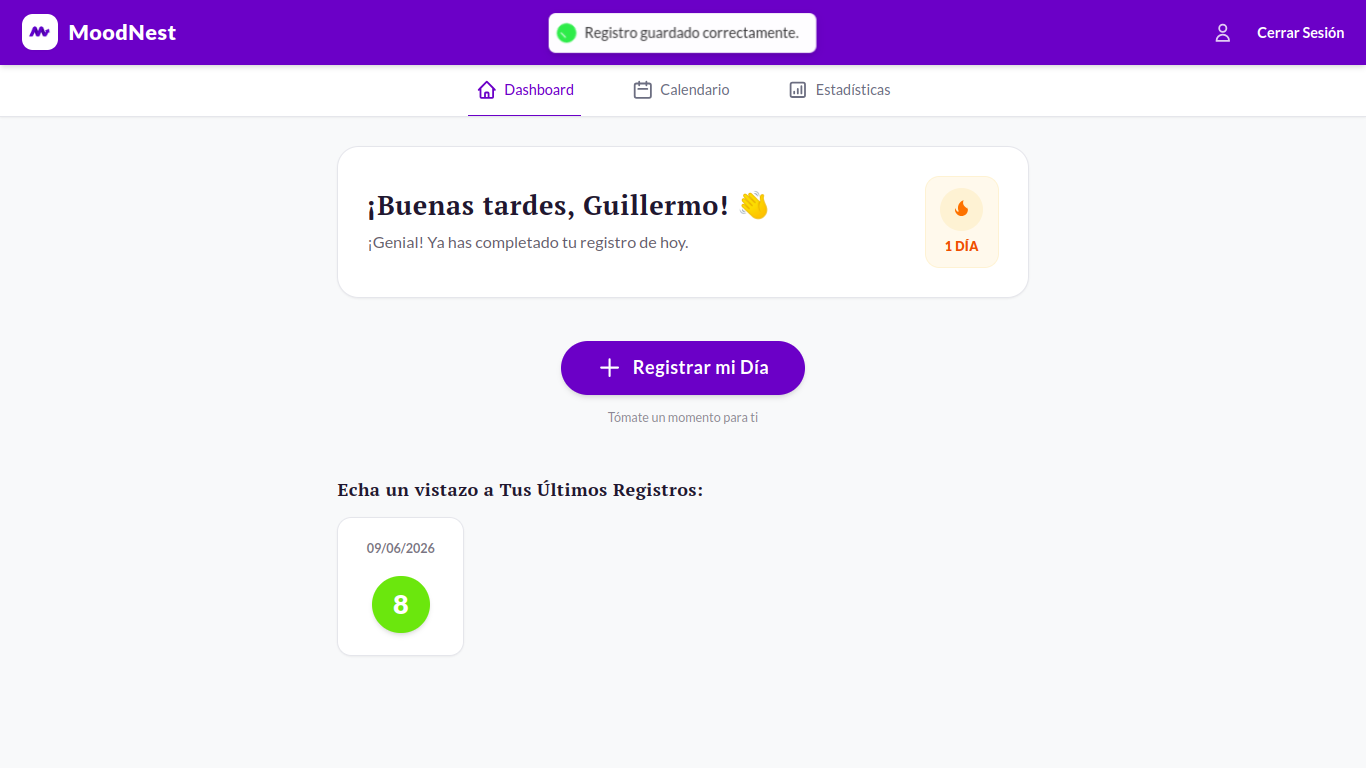
\includegraphics[width=0.85\textwidth]{Imagenes/pantalla_dashboard_postregistro.png}
    \caption{Estado del Dashboard tras consolidar el registro diario.}
    \label{fig:dashboard_post}
\end{figure}

Las actualizaciones automáticas del sistema visibles en este panel corresponden a:
\begin{itemize}
    \item \textbf{Actualización de Métricas Dinámicas:} El saludo felicita proactivamente al usuario por haber completado la jornada y el contador de racha incrementa su valor de forma inmediata a \texttt{1 día}.
    \item \textbf{Bloque de Últimos Registros:} En la parte final de la pantalla aparecerá una nueva tarjeta interactiva correspondiente al registro recién creado. Esta tarjeta visualiza la fecha formateada y la nota global encerrada en el color semántico asociado.
    \item \textbf{Visualización de Detalles:} Si el usuario interactúa haciendo clic sobre cualquiera de las tarjetas de las últimas entradas registradas, será redirigido hacia la pantalla de Historial y cargando los detalles del registro.
\end{itemize}

\subsection{Historial y Navegación Cronológica mensual}

La pantalla de Historial se plantea como un visor mensual interactivo estructurado en una disposición de doble columna responsiva. La Figura~\ref{fig:hist_con} muestra la inspección de un día con datos, y la Figura~\ref{fig:hist_sin} el estado ante un día vacío.

\begin{figure}[H]
    \centering
    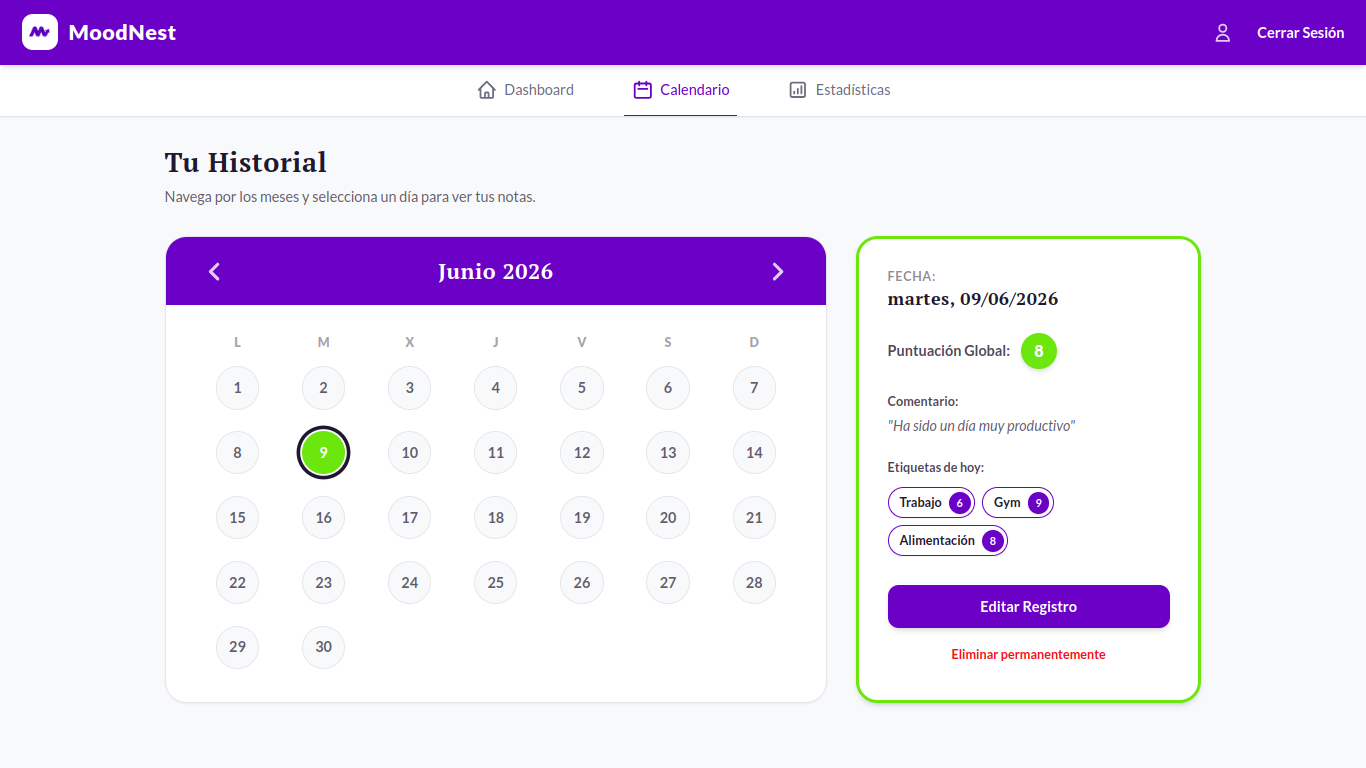
\includegraphics[width=0.85\textwidth]{Imagenes/pantalla_historial_postregistro.png}
    \caption{Vista de Historial: Inspección de un día con registro consolidado.}
    \label{fig:hist_con}
\end{figure}

\begin{figure}[H]
    \centering
    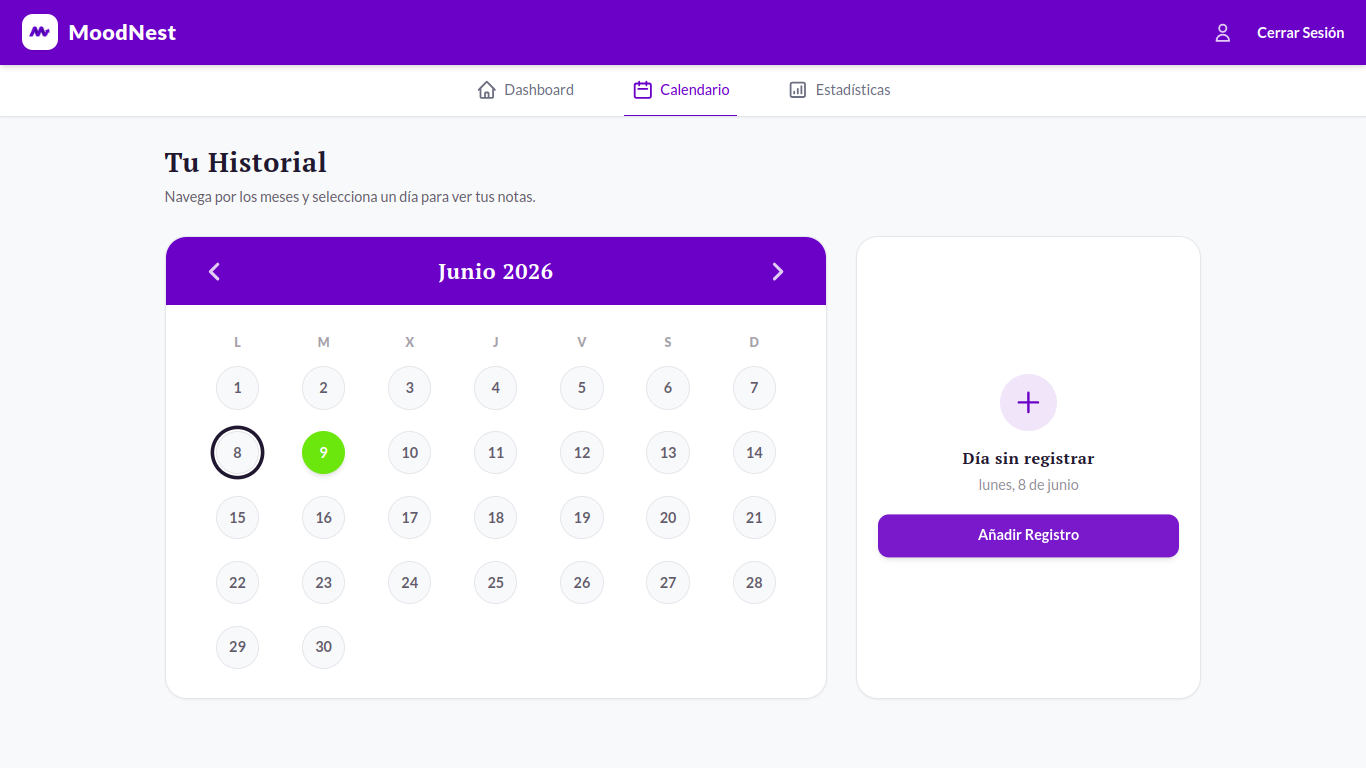
\includegraphics[width=0.85\textwidth]{Imagenes/pantalla_historial_diaSinRegistro.png}
    \caption{Vista de Historial: Panel derecho ante un día sin registro.}
    \label{fig:hist_sin}
\end{figure}

El comportamiento de este componente se rige por las siguientes interacciones:
\begin{itemize}
    \item \textbf{Navegación del Calendario (Columna Izquierda):} El usuario puede navegar entre meses utilizando las flechas del encabezado, para ver su historial completo de registros de un mes cualquiera. 
    \item \textbf{Panel Contextual de Inspección (Columna Derecha):} Al hacer clic sobre una celda del calendario, la columna derecha reacciona según la existencia de datos:
    \begin{itemize}
        \item \textbf{Día con registro:} Detalla la puntuación global, el comentario y el listado de etiquetas evaluadas. Habilita los botones para ``Editar'' y ``Eliminar'' dicho registro.
        \item \textbf{Día sin registro:} Muestra un estado vacío explicativo con un botón de inserción rápida configurado con la fecha de la celda seleccionada, para que el usuario añada un registro para ese día si así lo desea.
    \end{itemize}
\end{itemize}

\subsection{Panel de Configuración y Perfil de Usuario}

La vista de Perfil cede el gobierno absoluto de la aplicación al usuario autenticado, agrupando sus capacidades operativas en diferentes bloques de gestión (ver Figuras~\ref{fig:perf_ini} a~\ref{fig:perf_logout}).

\begin{figure}[H]
    \centering
    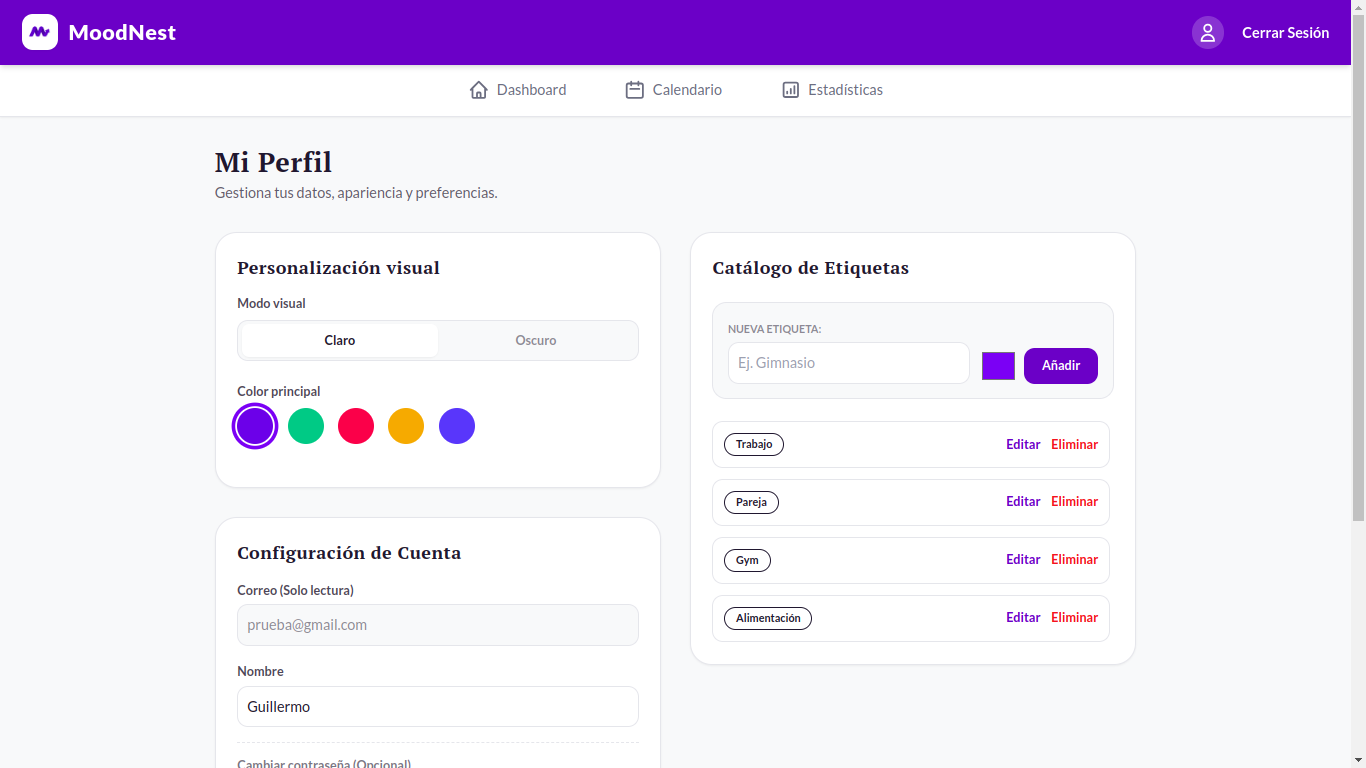
\includegraphics[width=0.85\textwidth]{Imagenes/pantalla_perfil_inicial.png}
    \caption{Vista general del panel de Perfil del usuario.}
    \label{fig:perf_ini}
\end{figure}

\begin{figure}[H]
    \centering
    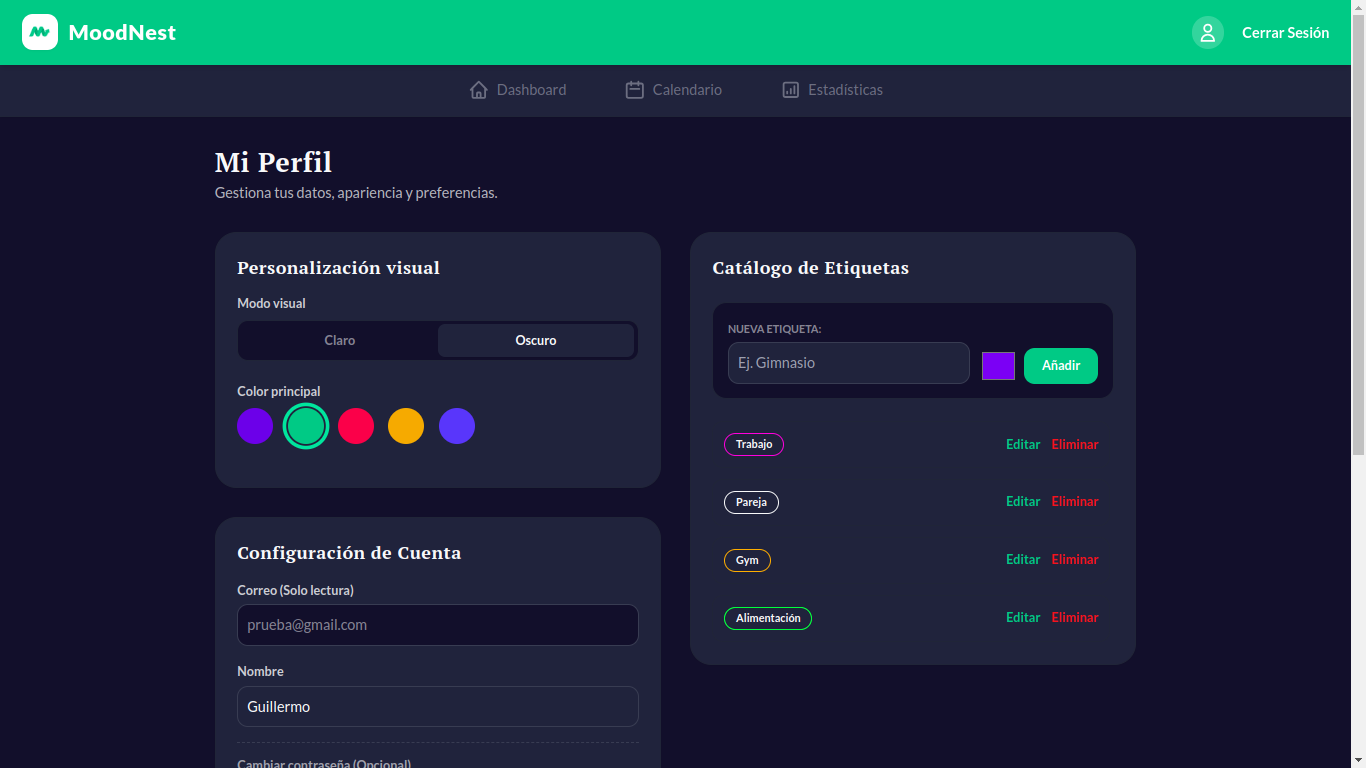
\includegraphics[width=0.85\textwidth]{Imagenes/pantalla_perfil_personalizarInterfaz.png}
    \caption{Widget de personalización estética de la interfaz (Tema y Color).}
    \label{fig:perf_inter}
\end{figure}

\begin{figure}[H]
    \centering
    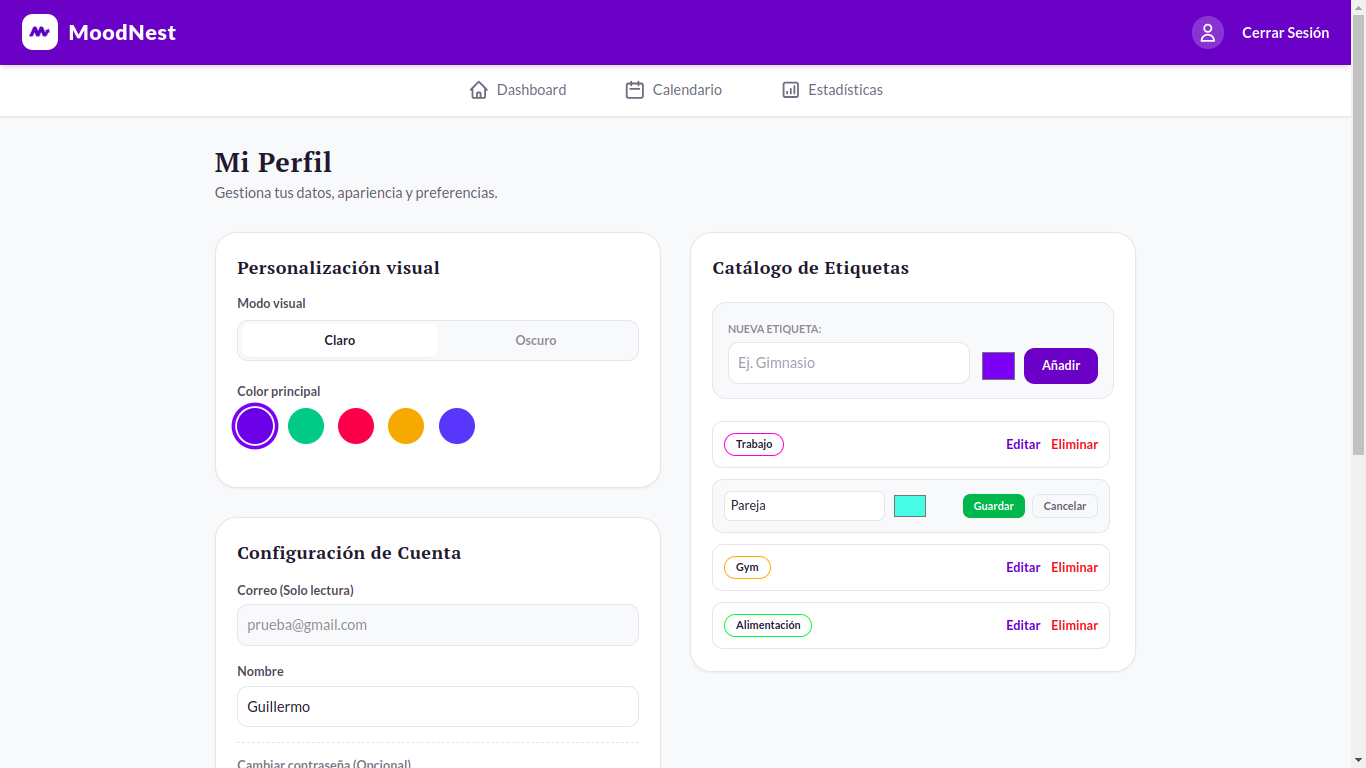
\includegraphics[width=0.85\textwidth]{Imagenes/pantalla_perfil_editarEtiqueta.png}
    \caption{Módulo de gestión y edición del catálogo de etiquetas.}
    \label{fig:perf_etiq}
\end{figure}

\begin{figure}[H]
    \centering
    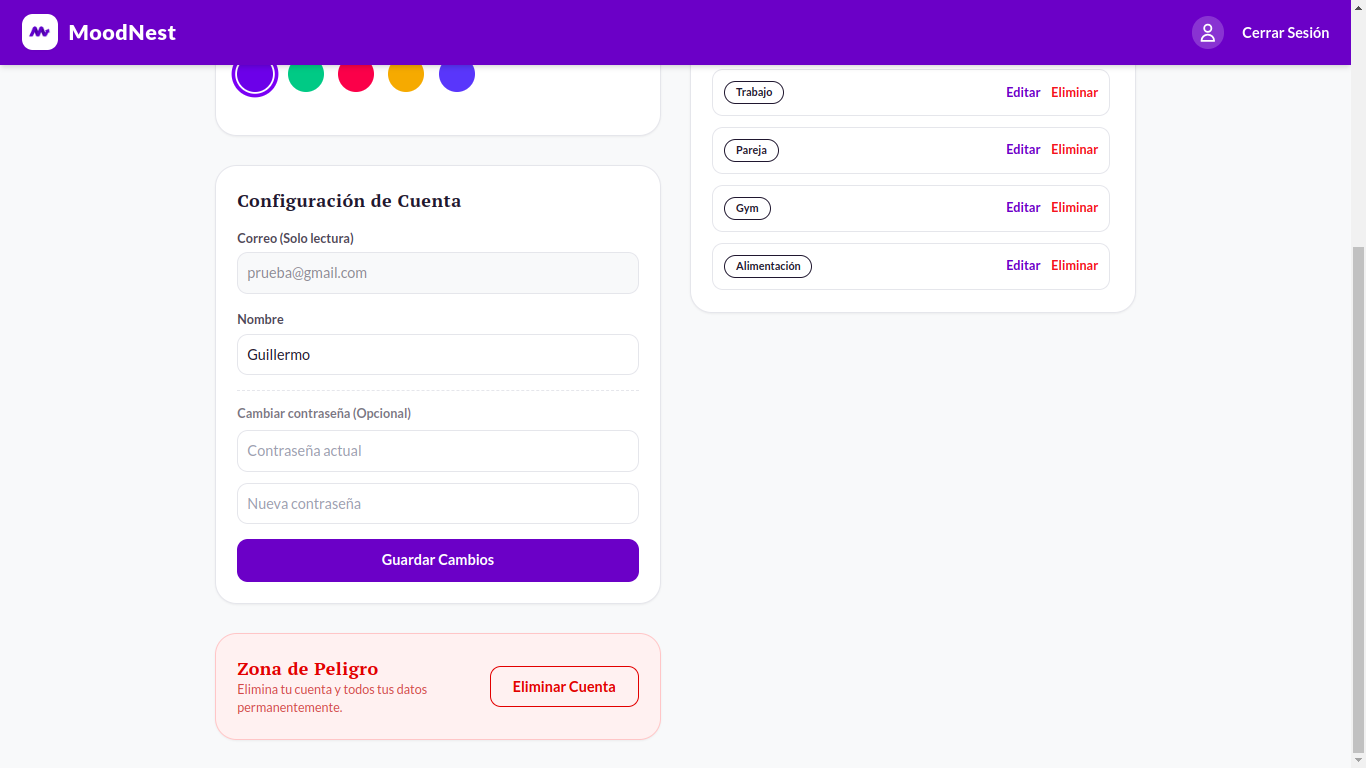
\includegraphics[width=0.85\textwidth]{Imagenes/pantalla_perfil_configuracionCuenta.png}
    \caption{Formularios de seguridad y actualización de credenciales.}
    \label{fig:perf_cuenta}
\end{figure}

Las funcionalidades desplegadas de forma atómica en este panel comprenden:
\begin{enumerate}
    \item \textbf{Personalización de la Interfaz (Figura~\ref{fig:perf_inter}):} Expone un conmutador semántico para alternar entre el Modo Claro y el Modo Oscuro, y una paleta de colores para reconfigurar el color principal de la interfaz.
    \item \textbf{Gestión de Catálogo de Etiquetas (Figura~\ref{fig:perf_etiq}):} Muestra el listado de las etiquetas personalizadas activas del usuario además de permitir la creación, edición y eliminación de las mismas mediante los botones de ``Añadir'', ``Editar'' y ``Eliminar''.
    \item \textbf{Configuración de la Cuenta (Figura~\ref{fig:perf_cuenta}):} Permite al usuario actualizar de manera independiente el nombre o la contraseña si así lo desea.
    \item \textbf{Eliminación de la Cuenta:} Acotado visualmente dentro de una ``Zona de Peligro'' (ver Figura~\ref{fig:perf_elim}). Al hacer clic en esta, el usuario deberá introducir su contraseña actual y así confirmar que realmente desea eliminar por completo su cuenta de MoodNest y todo su historial.
\end{enumerate}

\begin{figure}[H]
    \centering
    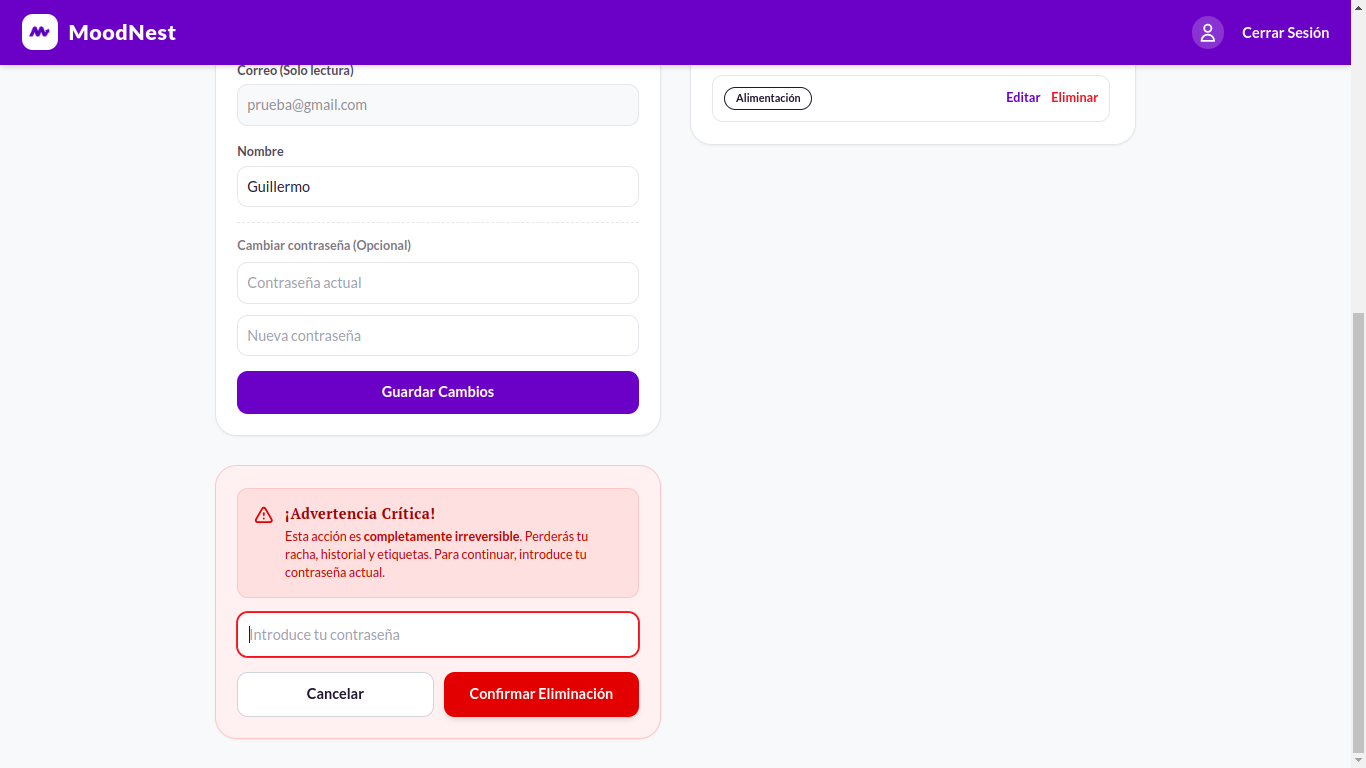
\includegraphics[width=0.85\textwidth]{Imagenes/pantalla_perfil_eliminarCuenta.png}
    \caption{Widget crítico de confirmación para la eliminación de la cuenta.}
    \label{fig:perf_elim}
\end{figure}

\subsection{Módulo Analítico y Estadísticas Avanzadas}

El panel de estadísticas representa el núcleo de MoodNest, traduciendo los registros diarios del usuario en conclusiones de valor sobre su bienestar.

\subsubsection{Comportamiento en Ausencia de Datos (Estado Vacío)}

Inicialmente, para usuario recién registrado en MoodNest que aún no cuenta con registros en su historial, la interfaz del sistema mostrará cuadros vacíos avisando al usuario de la falta de registros en su historial (ver Figuras~\ref{fig:est_vac1} y~\ref{fig:est_vac2}).

\begin{figure}[H]
    \centering
    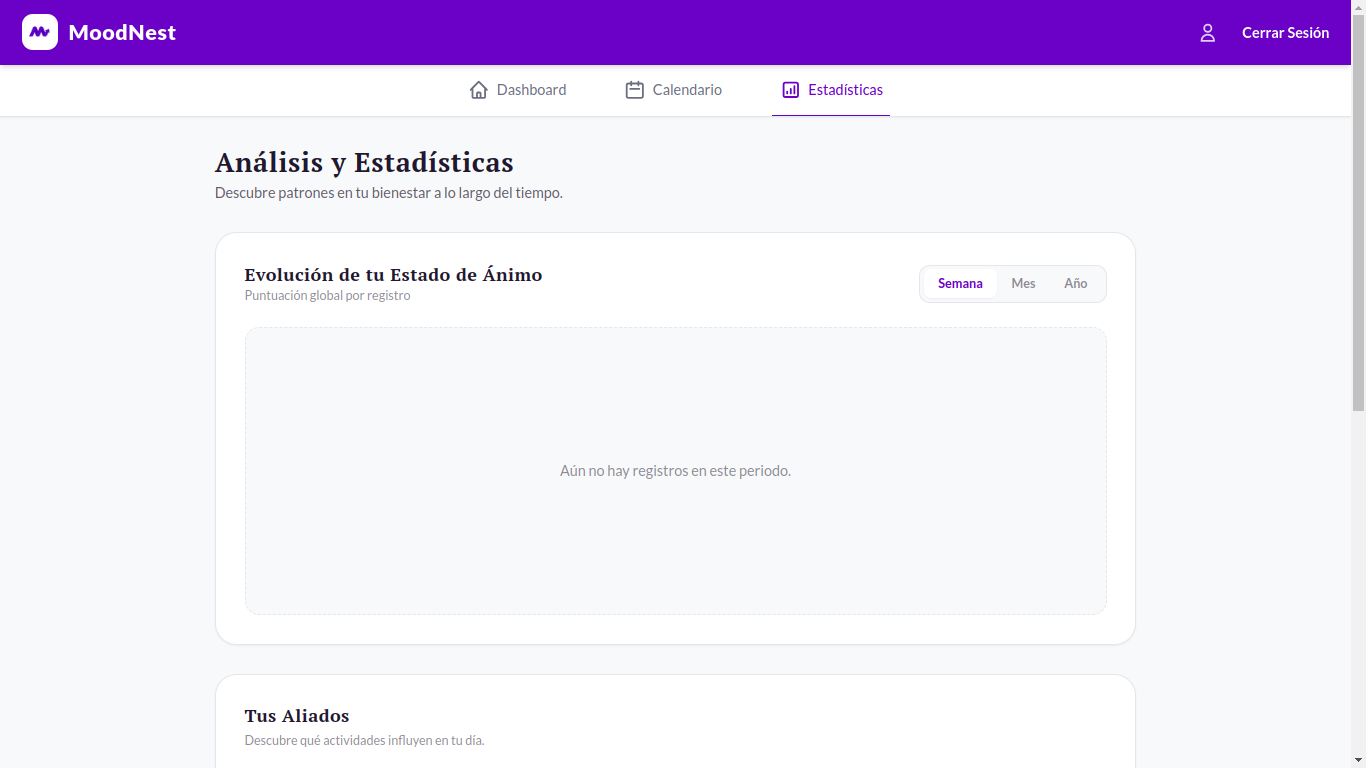
\includegraphics[width=0.85\textwidth]{Imagenes/pantalla_estadisticas_inicial_1.png}
    \caption{Estado inicial de estadísticas: Bloque cronológico superior vacío.}
    \label{fig:est_vac1}
\end{figure}

\begin{figure}[H]
    \centering
    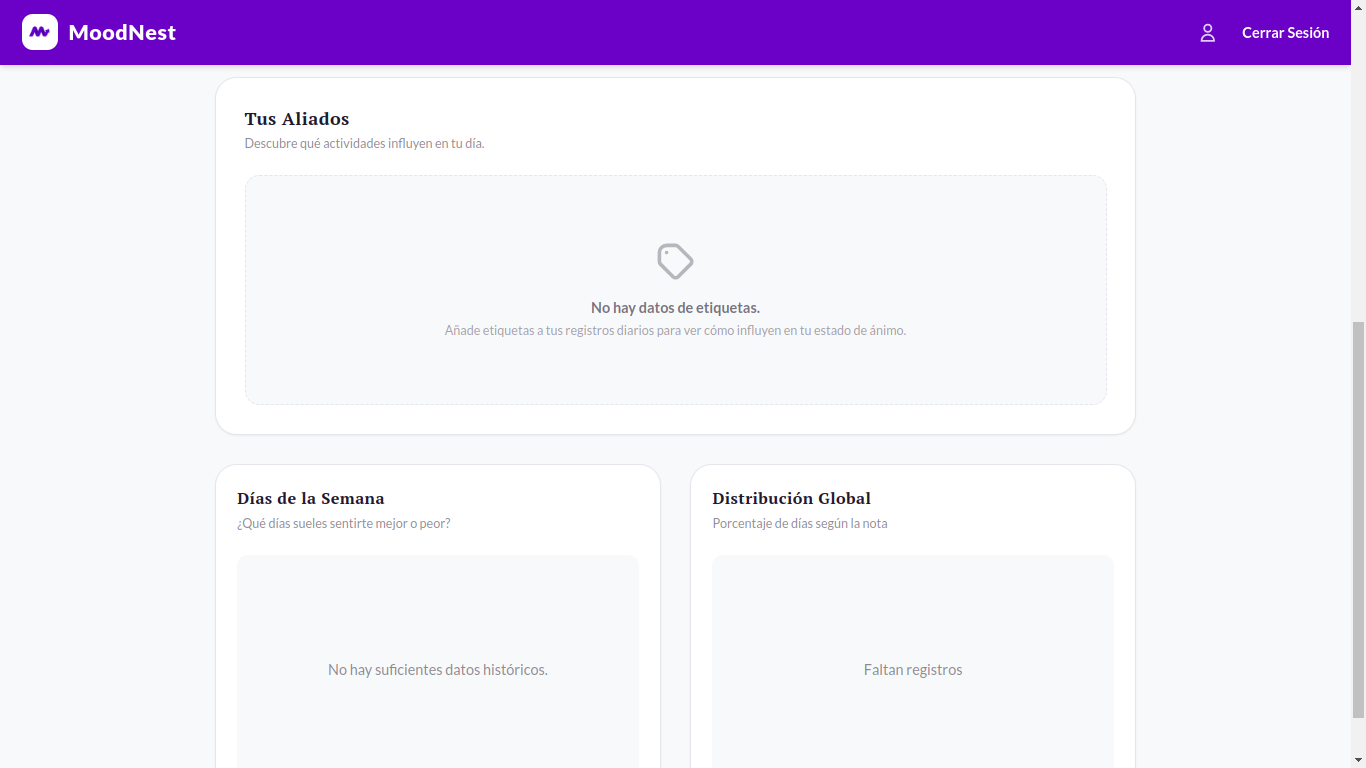
\includegraphics[width=0.85\textwidth]{Imagenes/pantalla_estadisticas_inicial_2.png}
    \caption{Estado inicial de estadísticas: Paneles analíticos de tags vacíos.}
    \label{fig:est_vac2}
\end{figure}

\subsubsection{Visualización Avanzada tras Uso Continuo}

Tras recopilar registros durante varios días o semanas, el módulo analítico se hidrata por completo y procesa todos y cada uno de los registros creados por el usuario, distribuyendo la información en tres secciones (ver Figuras~\ref{fig:est_sem} a~\ref{fig:est_dist}).

\begin{figure}[H]
    \centering
    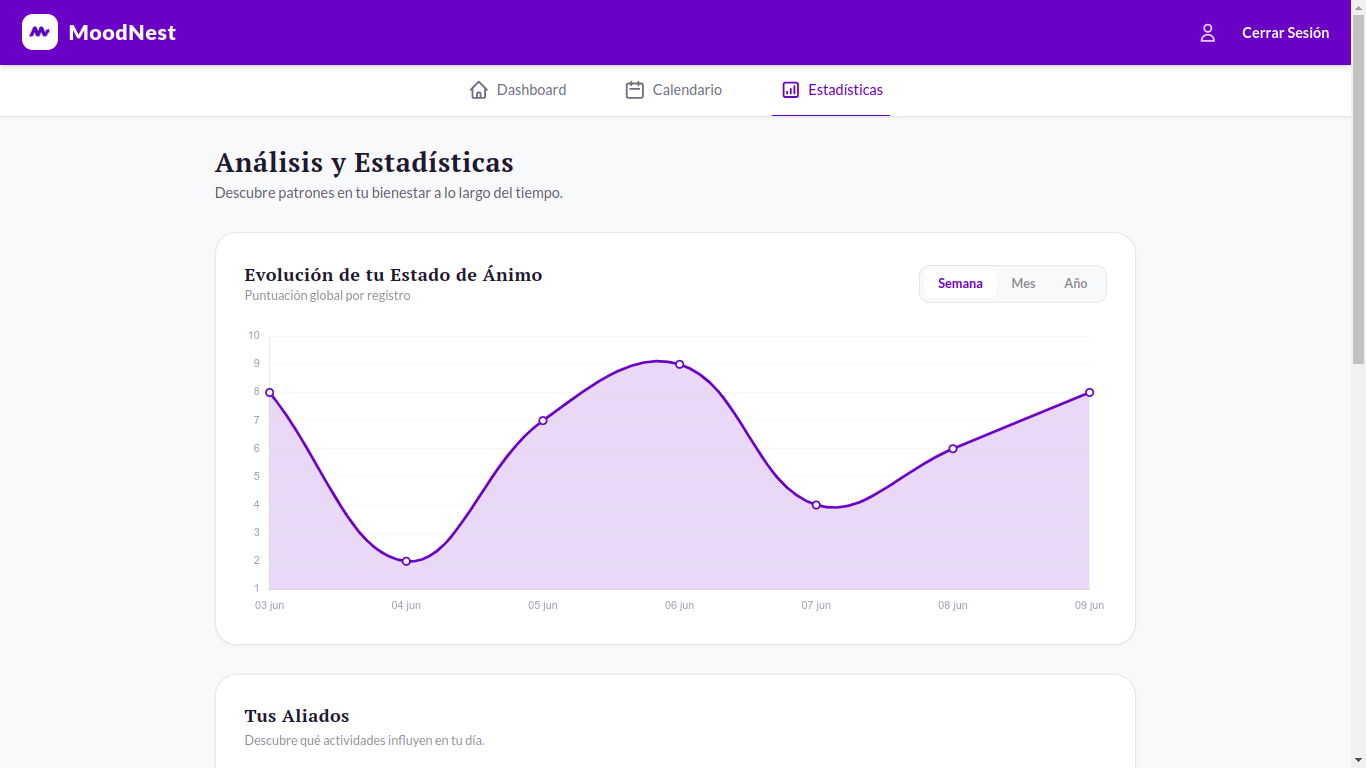
\includegraphics[width=0.85\textwidth]{Imagenes/pantalla_estadisticas_semanal.png}
    \caption{Gráfico de evolución temporal con filtro semanal activado.}
    \label{fig:est_sem}
\end{figure}

\begin{figure}[H]
    \centering
    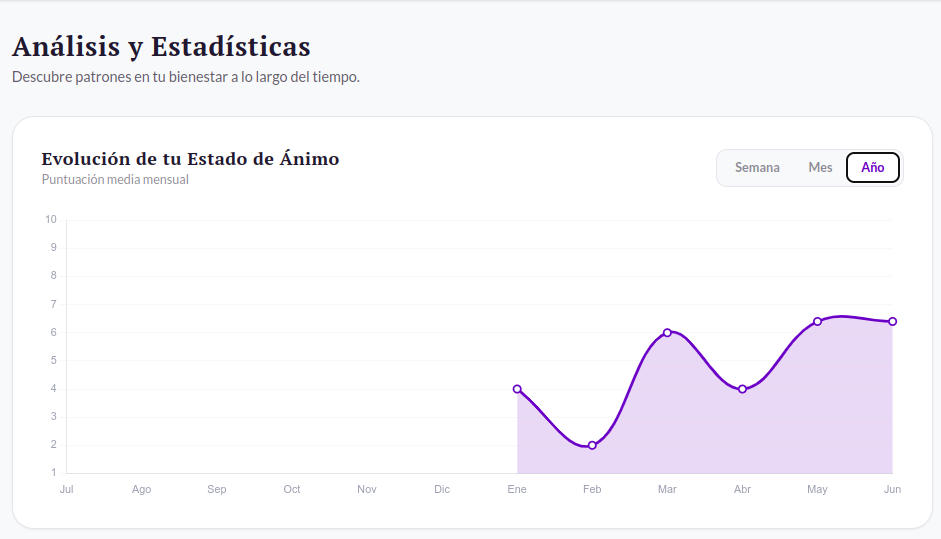
\includegraphics[width=0.85\textwidth]{Imagenes/pantalla_estadisticas_anual.png}
    \caption{Gráfico de evolución temporal con filtro anual activado.}
    \label{fig:est_anual}
\end{figure}

\begin{figure}[H]
    \centering
    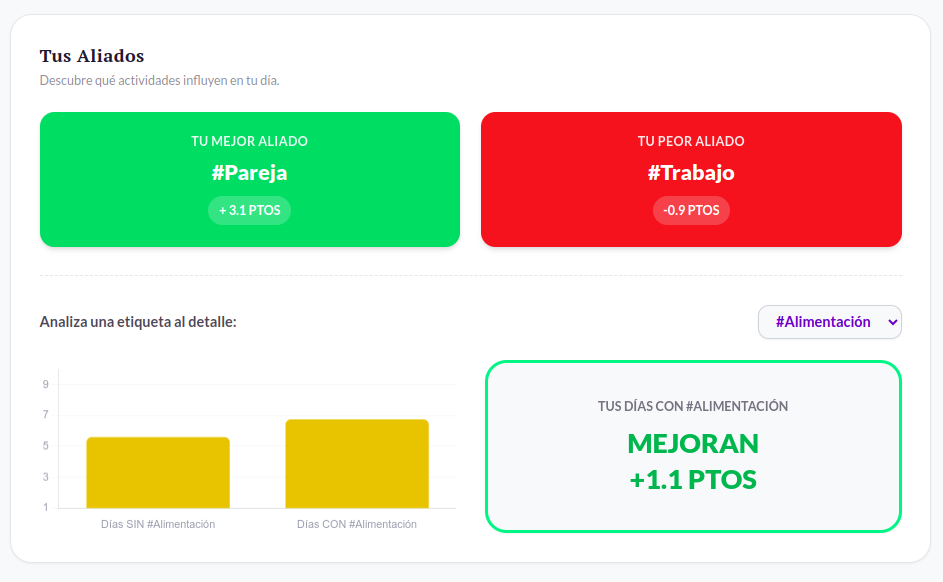
\includegraphics[width=0.85\textwidth]{Imagenes/pantalla_estadisticas_aliados.png}
    \caption{Métricas de correlación extrema de etiquetas (Aliados).}
    \label{fig:est_aliados}
\end{figure}

\begin{figure}[H]
    \centering
    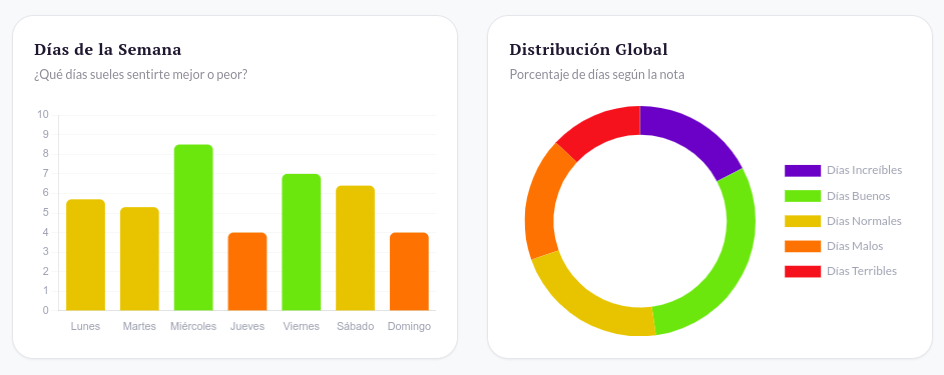
\includegraphics[width=0.85\textwidth]{Imagenes/pantalla_estadisticas_diasSemanaYPromedio.png}
    \caption{Distribuciones avanzadas: Barras por día y Anillo de promedio cualitativo.}
    \label{fig:est_dist}
\end{figure}

Los cuatro bloques funcionales operan bajo las siguientes premisas técnicas:
\begin{enumerate}
    \item \textbf{Evolución Temporal del Estado de Ánimo (Figuras~\ref{fig:est_sem} y~\ref{fig:est_anual}):} En esta sección se refleja la evolución temporal del estado de ánimo del usuario, pudiendo ver las fluctuaciones de su estado de ánimo a lo largo de la última semana, último mes y último año.
    \item \textbf{Módulo Central ``Tus Aliados'' (Figura~\ref{fig:est_aliados}):} En la parte superior de esta sección se muestran las dos etiquetas con mayor impacto en el estado de ánimo diario del usuario. En la parte izquierda se muestra la etiqueta con mayor impacto positivo y en la parte derecha se muestra la etiqueta con mayor impacto negativo, ambas acompañadas del impacto exacto en la puntuación diaria del usuario. Por otro lado, en la parte inferior el usuario puede valorar el impacto de una etiqueta concreta cualquiera, siempre y cuando exista al menos un registro con dicha etiqueta asociada y otro registro sin ella. La interfaz muestra un gráfico de barras comparativo entre la media de la puntuación global de los días sin la etiqueta y de los días con la etiqueta y justamente en la parte derecha, un mensaje dinámico sobre el resultado obtenido.
    \item \textbf{Distribuciones y Tendencias (Figura~\ref{fig:est_dist}):} En la parte final de las estadísticas, se encuentran dos gráficos. El de la izquierda permitirá al usuario conocer la tendencia de su estado de ánimo según el día de la semana, mientras que el de la derecha muestra la distribución porcentual del total de días registrados en el sistema agrupados por: días increíbles (puntuaciones de 9 y 10), buenos (puntuaciones de 7 y 8), normales (puntuaciones de 5 y 6), malos (puntuaciones de 3 y 4) y terribles (puntuaciones de 1 y 2).
\end{enumerate}

\subsection{Finalización de Sesión Segura}

El usuario autenticado dispone en todo momento del control para efectuar un cierre de sesión y asegurar así la privacidad de su información. Esta funcionalidad, se encuentra accesible en la zona lateral derecha de la barra superior de navegación, donde aparece exactamente el texto de ``Cerrar Sesión''.

Al interactuar con dicho elemento, la interfaz despliega una ventana modal de confirmación previa a la salida (ver Figura~\ref{fig:perf_logout}). Si el usuario ratifica la acción, el sistema mantendrá la privacidad del usuario y será redirigido nuevamente a la pantalla de bienvenida (Figura~\ref{fig:bienvenida}).


\begin{figure}[H]
    \centering
    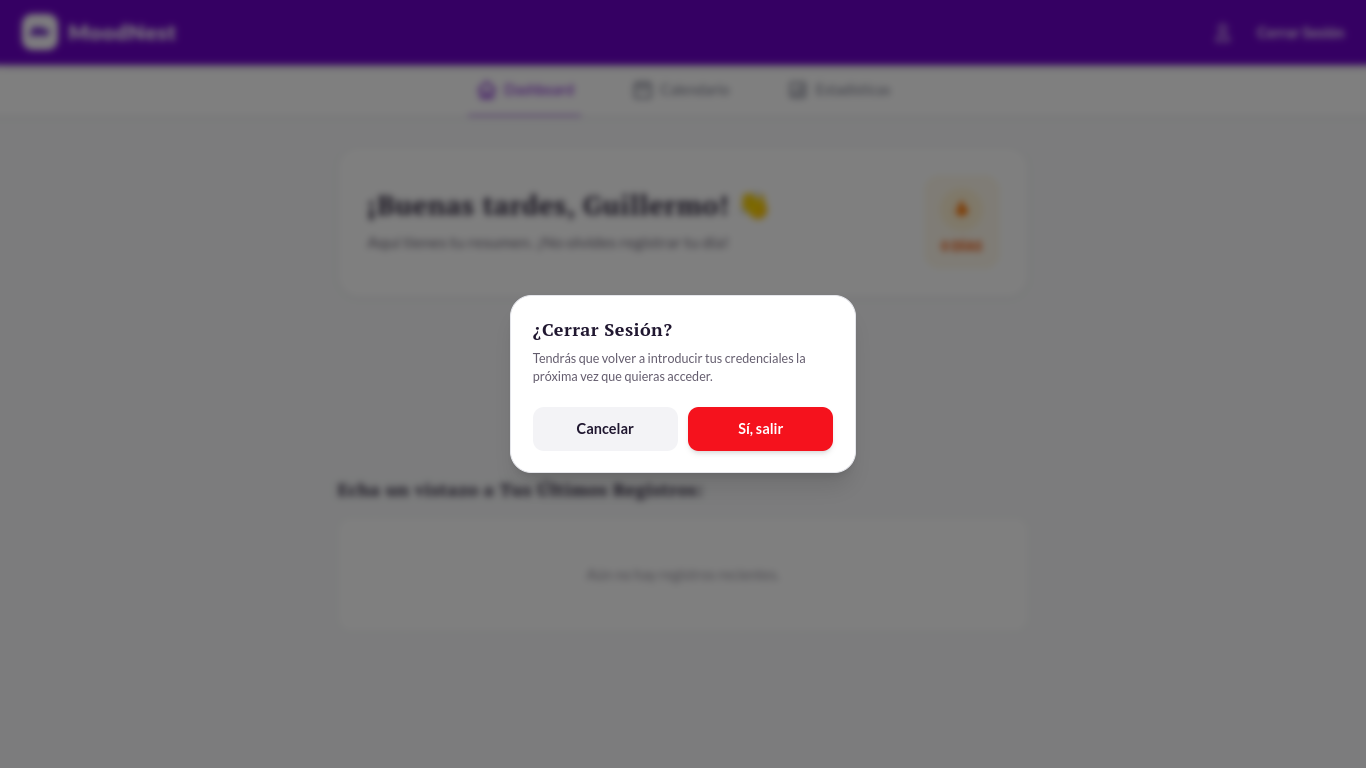
\includegraphics[width=0.85\textwidth]{Imagenes/pantalla_cerrar_sesion.png}
    \caption{Ventana modal de confirmación de Cierre de Sesión.}
    \label{fig:perf_logout}
\end{figure}
